\chapter{Search my protein in databases}
My choice was the \textbf{Discs Large MAGUK Scaffold Protein - DLG3}.
Where MAGUK is an abbreviation for \emph{membrane-associated guanylate kinase}.
I use Google for researching on-line, mainly found matching content on:
\begin{itemize}
\item \href{Uniprot.org}{http://www.uniprot.org/uniprot/Q62936}
\item \href{GeneCards.org}{http://www.genecards.org/cgi-bin/carddisp.pl?gene=DLG3}.
\end{itemize}

\section{What is its function?}
\begin{description}
\item[Entrez Gene Summary for DLG3 Gene]

    This gene encodes a member of the membrane-associated guanylate kinase protein family. The encoded protein may play a role in clustering of NMDA receptors at excitatory synapses. It may also negatively regulate cell proliferation through interaction with the C-terminal region of the adenomatosis polyposis coli tumor suppressor protein. Mutations in this gene have been associated with X-linked mental retardation. Alternatively spliced transcript variants have been described. [provided by RefSeq, Oct 2009]

\item[GeneCards Summary for DLG3 Gene]

DLG3 (Discs Large MAGUK Scaffold Protein 3) is a Protein Coding gene. Diseases associated with DLG3 include Non-Syndromic X-Linked Intellectual Disability and Partington Syndrome. Among its related pathways are Presynaptic function of Kainate receptors and L1CAM interactions. GO annotations related to this gene include ubiquitin protein ligase binding and protein C-terminus binding. An important paralog of this gene is DLG2.

\item[UniProtKB/Swiss-Prot for DLG3 Gene \url{DLG3_HUMAN,Q92796}]

Required for learning most likely through its role in synaptic plasticity following NMDA receptor signaling.

\item[Wikipedia]
Disks large homolog 3 (DLG3) also known as neuroendocrine-DLG or synapse-associated protein 102 (SAP-102) is a protein that in humans is encoded by the DLG3 gene.[3][4] DLG3 is a member of the membrane-associated guanylate kinase (MAGUK) superfamily of proteins.
\end{description}

\clearpage
\section{How many domains does it have and what kinds?}
According to Uniprot, DLG3 gene has \textbf{five} domains, namely the following:
\begin{description}
\item[PDZ 1] Position: 149 – 235
\item[PDZ 1] 244 – 330
\item[PDZ 1] 404 – 484	
\item[SH3] 519 – 589
\item[Guanylate kinase-like] 659 – 834	
\end{description}

\section{Which publication would you read if you started to work with this protein?}

In the first place I would like to read about \emph{Isolation of a gene (DLG3) encoding a second member of the discs-large family on chromosome}, by Smith \emph{et. al}~\cite{smith1996isolation}.
I would also consider reading Mutations in the \emph{DLG3} Gene Cause Nonsyndromic X-Linked Mental Retardation, by Tarpey \emph{et. al}~\cite{tarpey2004mutations}.

\section{Protein-protein interactions are particularly important for PDZ domains}

I have found the following literature in this topic, which are worth for further investigation:
\begin{description}
\item[PDZ domains and the organization of supramolecular complexes~\cite{sheng2001pdz}] PDZ domains are modular protein interaction domains that bind in a sequence-specific fashion to short C-terminal peptides or internal peptides that fold in a $\beta$-finger. The diversity of PDZ binding specificities can be explained by variable amino acids lining the peptide-binding groove of the PDZ domain. Abundantly represented in Caenorhabditis elegans, Drosophila melanogaster, and mammalian genomes, PDZ domains are frequently found in multiple copies or are associated with other protein-binding motifs in multidomain scaffold proteins. PDZ-containing proteins are typically involved in the assembly of supramolecular complexes that perform localized signaling functions at particular subcellular locations. Organization around a PDZ-based scaffold allows the stable localization of interacting proteins and enhances the rate and fidelity of signal transduction within the complex. Some PDZ-containing proteins are more dynamically regulated in distribution and may also be involved in the trafficking of interacting proteins within the cell.
\item[An evaluation of human protein-protein interaction data in the public domain~\cite{mathivanan2006evaluation}] Protein-protein interaction (PPI) databases have become a major resource for investigating biological networks and pathways in cells. A number of publicly available repositories for human PPIs are currently available. Each of these databases has their own unique features with a large variation in the type and depth of their annotations.
\end{description}

Especially I used the \emph{Uniprot} database to find which proteins interacts with my candidate. The result is depicted on a \emph{connection-graph} on Figure \ref{protprot}.

\begin{figure}
\centering
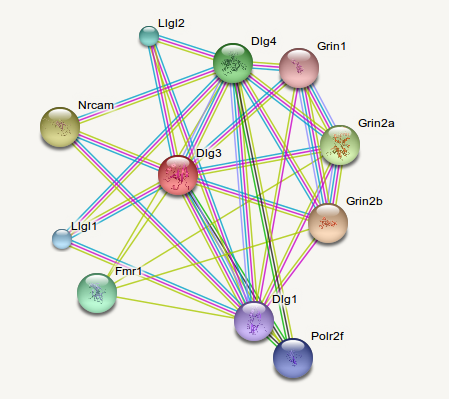
\includegraphics[width=\textwidth]{protprot.png}
\caption{\emph{Proteins containing PDZ
domains  influence the  function  of the PSD, synapses  and can  have a  clear  impact in multiple
neurological diseases.}
%
}
\label{protprot}
\end{figure}

\section{Could scientist determine a structure model for your protein yet?}

Yes, they could, a sequence model from the dabase \emph{\textsc{swiss-model}} is provided on Figure \ made with \href{http://biasmv.github.io/pv/}{PV - JavaScript Protein Viewer}

\begin{figure}
\centering
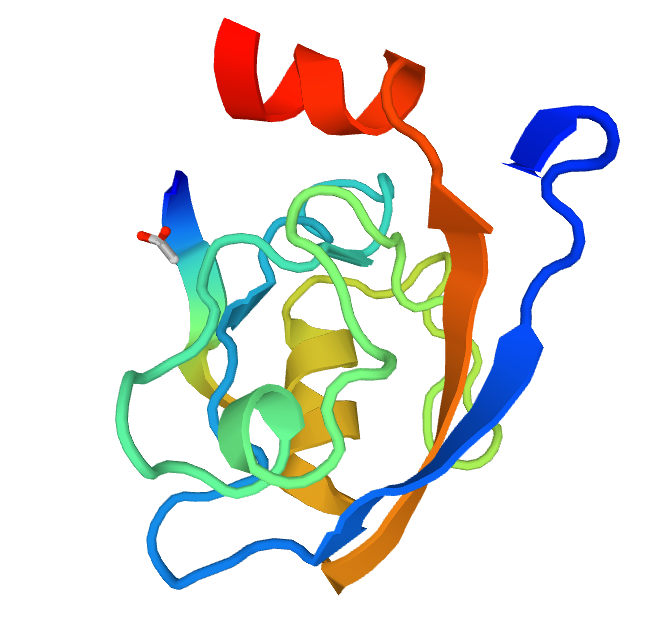
\includegraphics[width=\textwidth]{structure.png}
\caption{Sequential model of \url{DLG3_RAT}, from \href{https://modbase.compbio.ucsf.edu/modbase-cgi/model_details.cgi?queryfile=1479394245_9811&searchmode=default&displaymode=moddetail&referer=yes&snpflag=&}{\emph{\textsc{swiss-model}}}}
\label{structure}
\end{figure}

\section{Did you find anything else interesting?}
According to the results of my group mates, DLG3 is able to interact with much more protein than the others listen in the table.
It is interesting, because compared to the mentioned protein structures DLG3 has only three PDZ domains.